\documentclass[12pt, a4paper]{article}

% Pacchetti base essenziali
\usepackage[utf8]{inputenc}
\usepackage[T1]{fontenc}
\usepackage[italian]{babel}
\usepackage{graphicx}
\usepackage{float}
\usepackage{hyperref}
\usepackage{fancyhdr}
\usepackage{lastpage}
\usepackage{amssymb}
\usepackage{pifont}
\usepackage{xcolor}
\usepackage{booktabs}
\usepackage[most]{tcolorbox}
\usepackage{tikz}
\usetikzlibrary{shapes.geometric, arrows.meta, positioning, fit, calc}
\usepackage{array}
\usepackage{longtable}
\usepackage{enumitem}
\usepackage{tabularx}
\usepackage{multirow}

% Configurazione margini
\usepackage{geometry}
\geometry{
    a4paper,
    total={170mm,257mm},
    left=20mm,
    top=30mm,
    bottom=20mm,
    headheight=1.5cm,
    headsep=10mm,
    footskip=15mm,
}

% Rimuove l'indentazione dei paragrafi
\setlength{\parindent}{0pt}

% Configurazione header e footer
\pagestyle{fancy}
\fancyhf{}
\fancyhead[C]{\textbf{A.L.I.C.E. -- Documentazione di Progetto}}
\renewcommand{\headrulewidth}{0.4pt}
\fancyfoot[L]{Gruppo Flow}
\fancyfoot[R]{Pagina \thepage\ di \pageref{LastPage}}

\fancypagestyle{plain}{%
    \fancyhf{}
    \fancyhead[C]{\textbf{A.L.I.C.E. -- Documentazione di Progetto}}
    \renewcommand{\headrulewidth}{0.4pt}
    \fancyfoot[L]{Gruppo Flow}
    \fancyfoot[R]{Pagina \thepage\ di \pageref{LastPage}}
}

% Colori personalizzati
\definecolor{aliceblue}{RGB}{0, 102, 153}
\definecolor{alicelight}{RGB}{230, 242, 250}

% Configurazione hyperref
\hypersetup{
    colorlinks=true,
    linkcolor=aliceblue,
    urlcolor=aliceblue,
    citecolor=aliceblue,
}

\begin{document}

\begin{titlepage}
  \thispagestyle{empty}
  \centering
  \vspace*{3cm}

  {\Huge\bfseries A.L.I.C.E.\par}
  \vspace{0.5cm}
  {\large\textit{Assistente Intelligente per la Cura degli Elderly}\par}
  \vspace{2cm}

  {\LARGE Documentazione di Progetto\par}
  {\LARGE\bfseries Piattaforma Web per il Monitoraggio\par}
  {\LARGE\bfseries Remoto di Anziani\par}
  \vspace{2cm}

  {\large Anno Accademico:\par}
  {\large 2025/2026\par}
  \vspace{1cm}

  {\large Esame:\par}
  {\large PROGRAMMAZIONE PER IL WEB\par}
  \vspace{1.5cm}

  {\large\bfseries Realizzato da\par}
  \vspace{0.5cm}
  \begin{tabular}{l l l l}
    Manuel  & Manna         & 803080 & m.manna6@studenti.uniba.it       \\
    Alessio & Mininni       & 798191 & a.mininni14@studenti.uniba.it    \\
    Andrius & Tamuliunaite & 800256 & a.tamuliunaite@studenti.uniba.it \\
  \end{tabular}

  \vspace{1cm}
\end{titlepage}

\newpage

\tableofcontents
\newpage

% Inclusione delle sezioni
\section{Descrizione Informale del Contesto e degli Obiettivi}

La nostra applicazione mira a offrire una piattaforma web per il monitoraggio remoto e l'assistenza domiciliare di pazienti anziani. L'invecchiamento della popolazione richiede strumenti digitali accessibili, ma molte soluzioni esistenti risultano troppo complesse per l'utenza anziana oppure troppo frammentate per essere davvero utili agli operatori sanitari.

Il progetto \textbf{A.L.I.C.E.} nasce per colmare questo divario. Il sistema permette all'operatore sanitario di gestire i propri pazienti, assegnare esercizi fisici, configurare farmaci e monitorare umore, aderenza farmacologica e completamento degli esercizi. Il paziente, invece, utilizza un'interfaccia semplificata con card grandi, testi brevi e percorsi lineari.

\subsection{Doppia vista del sistema}

La piattaforma e' organizzata in due aree distinte:

\begin{itemize}
    \item \textbf{Area Operatore Sanitario:} comprende login, registrazione, dashboard con elenco pazienti, filtri per stato clinico, ricerca per nome, schede riepilogative e pagina di dettaglio del paziente. Nel dettaglio l'operatore puo' consultare metriche, storico umore, storico farmaci, storico esercizi, modificare i dati anagrafici, aggiungere o rimuovere farmaci ed esercizi.
    \item \textbf{Area Paziente Anziano:} comprende login, registrazione, home semplificata e tre funzionalita' principali: registrazione dell'umore quotidiano, esecuzione di esercizi fisici guidati passo-passo e conferma dell'assunzione dei farmaci.
\end{itemize}

\subsection{Funzionalita' principali}

Le funzionalita' effettivamente implementate nel progetto sono:

\begin{itemize}
    \item \textbf{Gestione utenza:} registrazione e login separati per operatore e paziente, con controllo del ruolo tramite Supabase Auth e tabella \texttt{profiles}.
    \item \textbf{Gestione pazienti:} ogni paziente e' associato a un operatore. L'operatore puo' visualizzare la lista, filtrarla, cercare per nome e accedere al dettaglio.
    \item \textbf{Gestione farmaci:} l'operatore inserisce nome, dosaggio e orario; il sistema calcola automaticamente la fascia oraria (\texttt{mattina}, \texttt{pranzo}, \texttt{sera}). Il paziente conferma l'assunzione giornaliera.
    \item \textbf{Gestione esercizi:} l'operatore crea esercizi fisici con durata, frequenza e passaggi guidati. Il paziente li esegue step-by-step e registra il completamento.
    \item \textbf{Monitoraggio umore:} il paziente registra ogni giorno il proprio umore scegliendo tra \texttt{triste}, \texttt{normale} e \texttt{felice}. L'operatore visualizza lo storico settimanale.
    \item \textbf{Suggerimento AI per l'operatore:} nella pagina di dettaglio paziente e' presente una route API che invia a Groq dati sintetici sul paziente e riceve una frase operativa di supporto.
\end{itemize}

\subsection{Obiettivi del progetto}

Gli obiettivi principali sono:

\begin{enumerate}
    \item \textbf{Semplificare l'interazione del paziente anziano}, riducendo la navigazione a pochi passaggi e usando componenti visivi chiari.
    \item \textbf{Centralizzare le informazioni utili all'operatore}, evitando che umore, farmaci ed esercizi siano gestiti in strumenti separati.
    \item \textbf{Misurare l'aderenza quotidiana}, tramite metriche percentuali su farmaci presi ed esercizi completati.
    \item \textbf{Migliorare la continuita' assistenziale}, permettendo all'operatore di controllare l'andamento del paziente anche tra una visita e l'altra.
    \item \textbf{Mantenere una struttura tecnica semplice}, basata su Next.js, React, Server Actions e Supabase, cosi' da rendere il progetto comprensibile e manutenibile.
\end{enumerate}

\newpage

\section{Individuazione degli Stakeholder e dei Goal}

\subsection{Stakeholder e Goal}

Gli stakeholder principali del sistema sono l'\textbf{Operatore Sanitario} e il \textbf{Paziente Anziano}. I due attori usano la stessa piattaforma, ma con obiettivi e livelli di complessita' diversi. L'operatore deve gestire e interpretare i dati; il paziente deve svolgere azioni quotidiane semplici.

\subsubsection{Operatore Sanitario / Caregiver}

L'operatore sanitario e' il professionista che segue uno o piu' pazienti. Attraverso la dashboard puo' consultare l'elenco dei pazienti assegnati, entrare nel dettaglio di ciascun paziente, aggiornare alcune informazioni, configurare farmaci ed esercizi e monitorare i log giornalieri.

\begin{table}[H]
\centering
\footnotesize
\renewcommand{\arraystretch}{1.25}
\begin{tabular}{|p{3.2cm}|p{4.4cm}|p{4.7cm}|c|c|c|c|}
\hline
\textbf{Stakeholder} & \textbf{Goal} & \textbf{Subgoal} & \textbf{C} & \textbf{R} & \textbf{U} & \textbf{D} \\
\hline
Operatore Sanitario & Gestione pazienti & Visualizza lista pazienti & & X & & \\
\cline{3-7}
 & & Modifica dati del paziente & & & X & \\
\cline{3-7}
 & & Consulta dettaglio e metriche & & X & & \\
\hline
Operatore Sanitario & Gestione farmaci & Aggiunge farmaco & X & & & \\
\cline{3-7}
 & & Visualizza farmaci assegnati & & X & & \\
\cline{3-7}
 & & Elimina farmaco & & & & X \\
\hline
Operatore Sanitario & Gestione esercizi & Crea esercizio con step & X & & & \\
\cline{3-7}
 & & Visualizza esercizi assegnati & & X & & \\
\cline{3-7}
 & & Elimina esercizio & & & & X \\
\hline
Operatore Sanitario & Monitoraggio & Consulta umore, farmaci ed esercizi & & X & & \\
\cline{3-7}
 & & Richiede suggerimento AI & X & & & \\
\hline
\end{tabular}
\caption{Goal e operazioni CRUD dell'Operatore Sanitario}
\label{tab:goal-operatore}
\end{table}

\subsubsection{Paziente Anziano}

Il paziente anziano usa l'applicazione per comunicare poche informazioni essenziali. Non gestisce il proprio piano terapeutico, ma interagisce con quanto configurato dall'operatore: vede i farmaci, conferma l'assunzione, vede gli esercizi, li completa e registra l'umore del giorno.

\begin{table}[H]
\centering
\footnotesize
\renewcommand{\arraystretch}{1.25}
\begin{tabular}{|p{3.2cm}|p{4.2cm}|p{4.9cm}|c|c|c|c|}
\hline
\textbf{Stakeholder} & \textbf{Goal} & \textbf{Subgoal} & \textbf{C} & \textbf{R} & \textbf{U} & \textbf{D} \\
\hline
Paziente Anziano & Accesso & Login e registrazione associata a un operatore & X & X & & \\
\hline
Paziente Anziano & Umore & Registra o aggiorna umore quotidiano & X & X & X & \\
\hline
Paziente Anziano & Esercizi fisici & Visualizza lista esercizi & & X & & \\
\cline{3-7}
 & & Completa esercizio guidato & X & X & & \\
\hline
Paziente Anziano & Farmaci & Visualizza farmaci per fascia oraria & & X & & \\
\cline{3-7}
 & & Conferma o annulla assunzione & X & X & X & \\
\hline
\end{tabular}
\caption{Goal e operazioni CRUD del Paziente Anziano}
\label{tab:goal-paziente}
\end{table}

\newpage
\subsection{Diagramma di Contesto}

Il diagramma di contesto rappresenta A.L.I.C.E. come una scatola nera posta al centro dell'interazione tra utenti e servizi esterni. L'operatore sanitario invia al sistema configurazioni e aggiornamenti relativi a pazienti, farmaci ed esercizi; in cambio riceve dashboard, metriche, storico dei log e suggerimenti sintetici. Il paziente invia conferme giornaliere, completamenti degli esercizi e valore dell'umore; in cambio riceve una home semplificata, l'elenco delle attivita' e le istruzioni operative.

Sul lato dei servizi, Supabase fornisce autenticazione, persistenza dei dati e controllo di visibilita' tramite Row Level Security. La Groq API viene usata solo dalla route server-side dedicata al suggerimento AI: il browser non riceve la chiave del servizio esterno e il testo generato e' destinato all'operatore.

\begin{figure}[H]
\centering
\begin{tikzpicture}[
    entity/.style={rectangle, draw=aliceblue, fill=alicelight, thick, minimum width=3.5cm, minimum height=1cm, align=center, font=\small\bfseries},
    system/.style={rectangle, draw=aliceblue, fill=aliceblue!15, thick, rounded corners=6pt, minimum width=4.5cm, minimum height=2cm, align=center, font=\large\bfseries},
    service/.style={rectangle, draw=alicegreen, fill=green!8, thick, rounded corners=4pt, minimum width=3.6cm, minimum height=1cm, align=center, font=\small\bfseries},
    flow/.style={-{Stealth[length=2.5mm]}, thick, color=aliceblue},
    flowlabel/.style={font=\scriptsize, fill=white, inner sep=2pt, align=center},
]
\node[system] (alice) {A.L.I.C.E.\\Applicazione Web};
\node[entity, above left=2.4cm and 2.8cm of alice] (operatore) {Operatore\\Sanitario};
\node[entity, above right=2.4cm and 2.8cm of alice] (paziente) {Paziente\\Anziano};
\node[service, below left=2.2cm and 1.8cm of alice] (supabase) {Supabase\\Auth + PostgreSQL};
\node[service, below right=2.2cm and 1.8cm of alice] (groq) {Groq API\\AI};

\draw[flow] (operatore) -- node[flowlabel] {configura pazienti,\\farmaci, esercizi} (alice);
\draw[flow] (alice) -- node[flowlabel] {dashboard, metriche,\\storici, suggerimento} (operatore);
\draw[flow] (paziente) -- node[flowlabel] {umore, conferme,\\completamenti} (alice);
\draw[flow] (alice) -- node[flowlabel] {home, farmaci,\\esercizi guidati} (paziente);
\draw[flow] (alice) -- node[flowlabel] {sessioni e query} (supabase);
\draw[flow] (supabase) -- node[flowlabel] {dati e RLS} (alice);
\draw[flow] (alice) -- node[flowlabel] {dati sintetici} (groq);
\draw[flow] (groq) -- node[flowlabel] {frase operativa} (alice);
\end{tikzpicture}
\caption{Diagramma di contesto del sistema A.L.I.C.E.}
\label{fig:contesto}
\end{figure}

\subsection{Scambio di Valore}

\begin{figure}[H]
\centering
\begin{tikzpicture}[
    system/.style={circle, draw=aliceblue, fill=aliceblue!12, thick, minimum size=2.7cm, align=center, font=\bfseries},
    ai/.style={rectangle, draw=aliceorange, fill=aliceorange!10, thick, rounded corners=4pt, minimum width=2.8cm, minimum height=0.8cm, align=center, font=\scriptsize\bfseries},
    flow/.style={-{Stealth[length=2.5mm]}, thick},
    label/.style={font=\scriptsize, fill=white, inner sep=2pt, align=center},
]

\node[system] (alice) at (0, 0) {A.L.I.C.E.};
\node[ai] (ai) at (0, -2.3) {Feature AI\\Suggerimento};

% omino operatore
\coordinate (op) at (-5.5, 0);
\draw[aliceblue, thick] ($(op)+(0,0.8)$) circle (0.35);
\draw[aliceblue, thick] ($(op)+(0,0.45)$) -- ($(op)+(0,-0.55)$);
\draw[aliceblue, thick] ($(op)+(-0.65,0.1)$) -- ($(op)+(0.65,0.1)$);
\draw[aliceblue, thick] ($(op)+(0,-0.55)$) -- ($(op)+(-0.55,-1.25)$);
\draw[aliceblue, thick] ($(op)+(0,-0.55)$) -- ($(op)+(0.55,-1.25)$);
\node[align=center, font=\small\bfseries] at ($(op)+(0,-1.75)$) {Operatore\\Sanitario};

% omino paziente
\coordinate (pz) at (5.5, 0);
\draw[alicegreen, thick] ($(pz)+(0,0.8)$) circle (0.35);
\draw[alicegreen, thick] ($(pz)+(0,0.45)$) -- ($(pz)+(0,-0.55)$);
\draw[alicegreen, thick] ($(pz)+(-0.65,0.1)$) -- ($(pz)+(0.65,0.1)$);
\draw[alicegreen, thick] ($(pz)+(0,-0.55)$) -- ($(pz)+(-0.55,-1.25)$);
\draw[alicegreen, thick] ($(pz)+(0,-0.55)$) -- ($(pz)+(0.55,-1.25)$);
\node[align=center, font=\small\bfseries] at ($(pz)+(0,-1.75)$) {Paziente\\Anziano};

\draw[flow, color=aliceblue] (-4.5, 0.7) -- node[label] {pazienti, farmaci,\\esercizi} (-1.45, 0.75);
\draw[flow, color=aliceblue] (-1.45, -0.7) -- node[label] {metriche, storico,\\supporto decisionale} (-4.5, -0.7);
\draw[flow, color=alicegreen] (4.5, 0.7) -- node[label] {umore, conferme,\\completamenti} (1.45, 0.75);
\draw[flow, color=alicegreen] (1.45, -0.7) -- node[label] {interfaccia semplice,\\routine giornaliera} (4.5, -0.7);
\draw[flow, color=aliceorange] (alice) -- node[label, right] {genera frase\\per operatore} (ai);
\end{tikzpicture}
\caption{Scambio di valore con Operatore, Paziente e feature AI}
\label{fig:scambio-valore}
\end{figure}

\newpage

\section{Stato dell'Arte, Analisi della Concorrenza e Analisi ``Make or Buy''}

\subsection{Stato dell'Arte}

Il settore dell'assistenza domiciliare per anziani dispone oggi di numerose soluzioni digitali, ma spesso ciascuna copre un solo bisogno: promemoria farmacologici, teleassistenza, raccolta parametri o dashboard cliniche. A.L.I.C.E. si colloca in una zona intermedia: non vuole sostituire una cartella clinica professionale, ma integrare in una singola applicazione web le azioni quotidiane piu' rilevanti per il monitoraggio remoto.

Le tecnologie moderne rendono questo approccio sostenibile:

\begin{itemize}
    \item \textbf{Framework full-stack:} Next.js permette di gestire pagine, rendering server-side, Server Components, Server Actions e route API nello stesso progetto.
    \item \textbf{Backend-as-a-Service:} Supabase riduce la complessita' del backend fornendo PostgreSQL, autenticazione, API auto-generate e Row Level Security.
    \item \textbf{Interfacce responsive:} l'applicazione e' utilizzabile da browser desktop e tablet, senza installazione.
    \item \textbf{AI come supporto operativo:} una route server-side puo' inviare dati sintetici a un modello esterno e ricevere suggerimenti testuali per l'operatore.
\end{itemize}

\subsection{Analisi della Concorrenza}

Sono stati considerati due competitor principali, gia' presenti nella versione finale del documento dello scorso appello.

\subsubsection{MyTherapy}

MyTherapy e' un'applicazione focalizzata sull'aderenza terapeutica. Gestisce promemoria per i farmaci, consente il tracciamento di parametri vitali e produce report utilizzabili dal personale medico. Il suo limite, rispetto ad A.L.I.C.E., e' la focalizzazione quasi esclusiva sulla terapia farmacologica: non offre una dashboard costruita attorno a esercizi fisici guidati e umore quotidiano con una vista anziano estremamente semplificata.

\subsubsection{ADiLife}

ADiLife e' un sistema professionale di teleassistenza per strutture sanitarie. Offre robustezza infrastrutturale e hardware dedicato, ma risulta piu' costoso e meno adatto a un progetto universitario basato su web app e strumenti open source. Il focus e' piu' orientato all'emergenza e al monitoraggio clinico professionale che alla routine quotidiana del paziente.

\begin{table}[H]
\centering
\footnotesize
\renewcommand{\arraystretch}{1.3}
\begin{tabular}{|p{3cm}|c|c|c|c|}
\hline
\textbf{Piattaforma} & \textbf{Farmaci} & \textbf{Esercizi} & \textbf{Umore} & \textbf{Dashboard operatore} \\
\hline
MyTherapy & \textcolor{green}{\checkmark} & \textcolor{red}{$\times$} & \textcolor{red}{$\times$} & Parziale \\
\hline
ADiLife & \textcolor{green}{\checkmark} & \textcolor{red}{$\times$} & \textcolor{red}{$\times$} & \textcolor{green}{\checkmark} \\
\hline
A.L.I.C.E. & \textcolor{green}{\checkmark} & \textcolor{green}{\checkmark} & \textcolor{green}{\checkmark} & \textcolor{green}{\checkmark} \\
\hline
\end{tabular}
\caption{Confronto sintetico tra A.L.I.C.E. e competitor}
\label{tab:confronto-competitor}
\end{table}

\subsection{Analisi ``Make or Buy''}

\begin{table}[H]
\centering
\renewcommand{\arraystretch}{1.35}
\begin{tabularx}{\textwidth}{|p{3cm}|X|X|}
\hline
\textbf{Criterio} & \textbf{Make} & \textbf{Buy} \\
\hline
Personalizzazione & Interfaccia progettata per due ruoli: operatore e paziente anziano. & Personalizzazione limitata ai vincoli del prodotto commerciale. \\
\hline
Costi & Bassi in fase iniziale grazie a Next.js, React e Supabase. & Licenze e costi di integrazione piu' alti. \\
\hline
Integrazione & Farmaci, esercizi, umore e dashboard nello stesso modello dati. & Spesso richiede piu' strumenti separati. \\
\hline
Controllo tecnico & Pieno controllo del codice, dello schema e delle regole RLS. & Dipendenza dal vendor. \\
\hline
\end{tabularx}
\caption{Analisi comparativa Make vs Buy}
\label{tab:make-or-buy}
\end{table}

La scelta finale e' \textbf{Make}: lo sviluppo interno consente di mantenere il progetto coerente con gli obiettivi didattici, con l'accessibilita' richiesta e con la reale struttura software implementata.

\newpage

\section{Modello Informativo}

\subsection{Diagramma EER}

l diagramma Entity-Enhanced Relationship descrive la struttura concettuale della base di dati. Le entità sono state individuate a partire dall'analisi dei requisiti funzionali e riflettono lo schema effettivamente implementato su Supabase (PostgreSQL).

\begin{figure}[H]
\centering
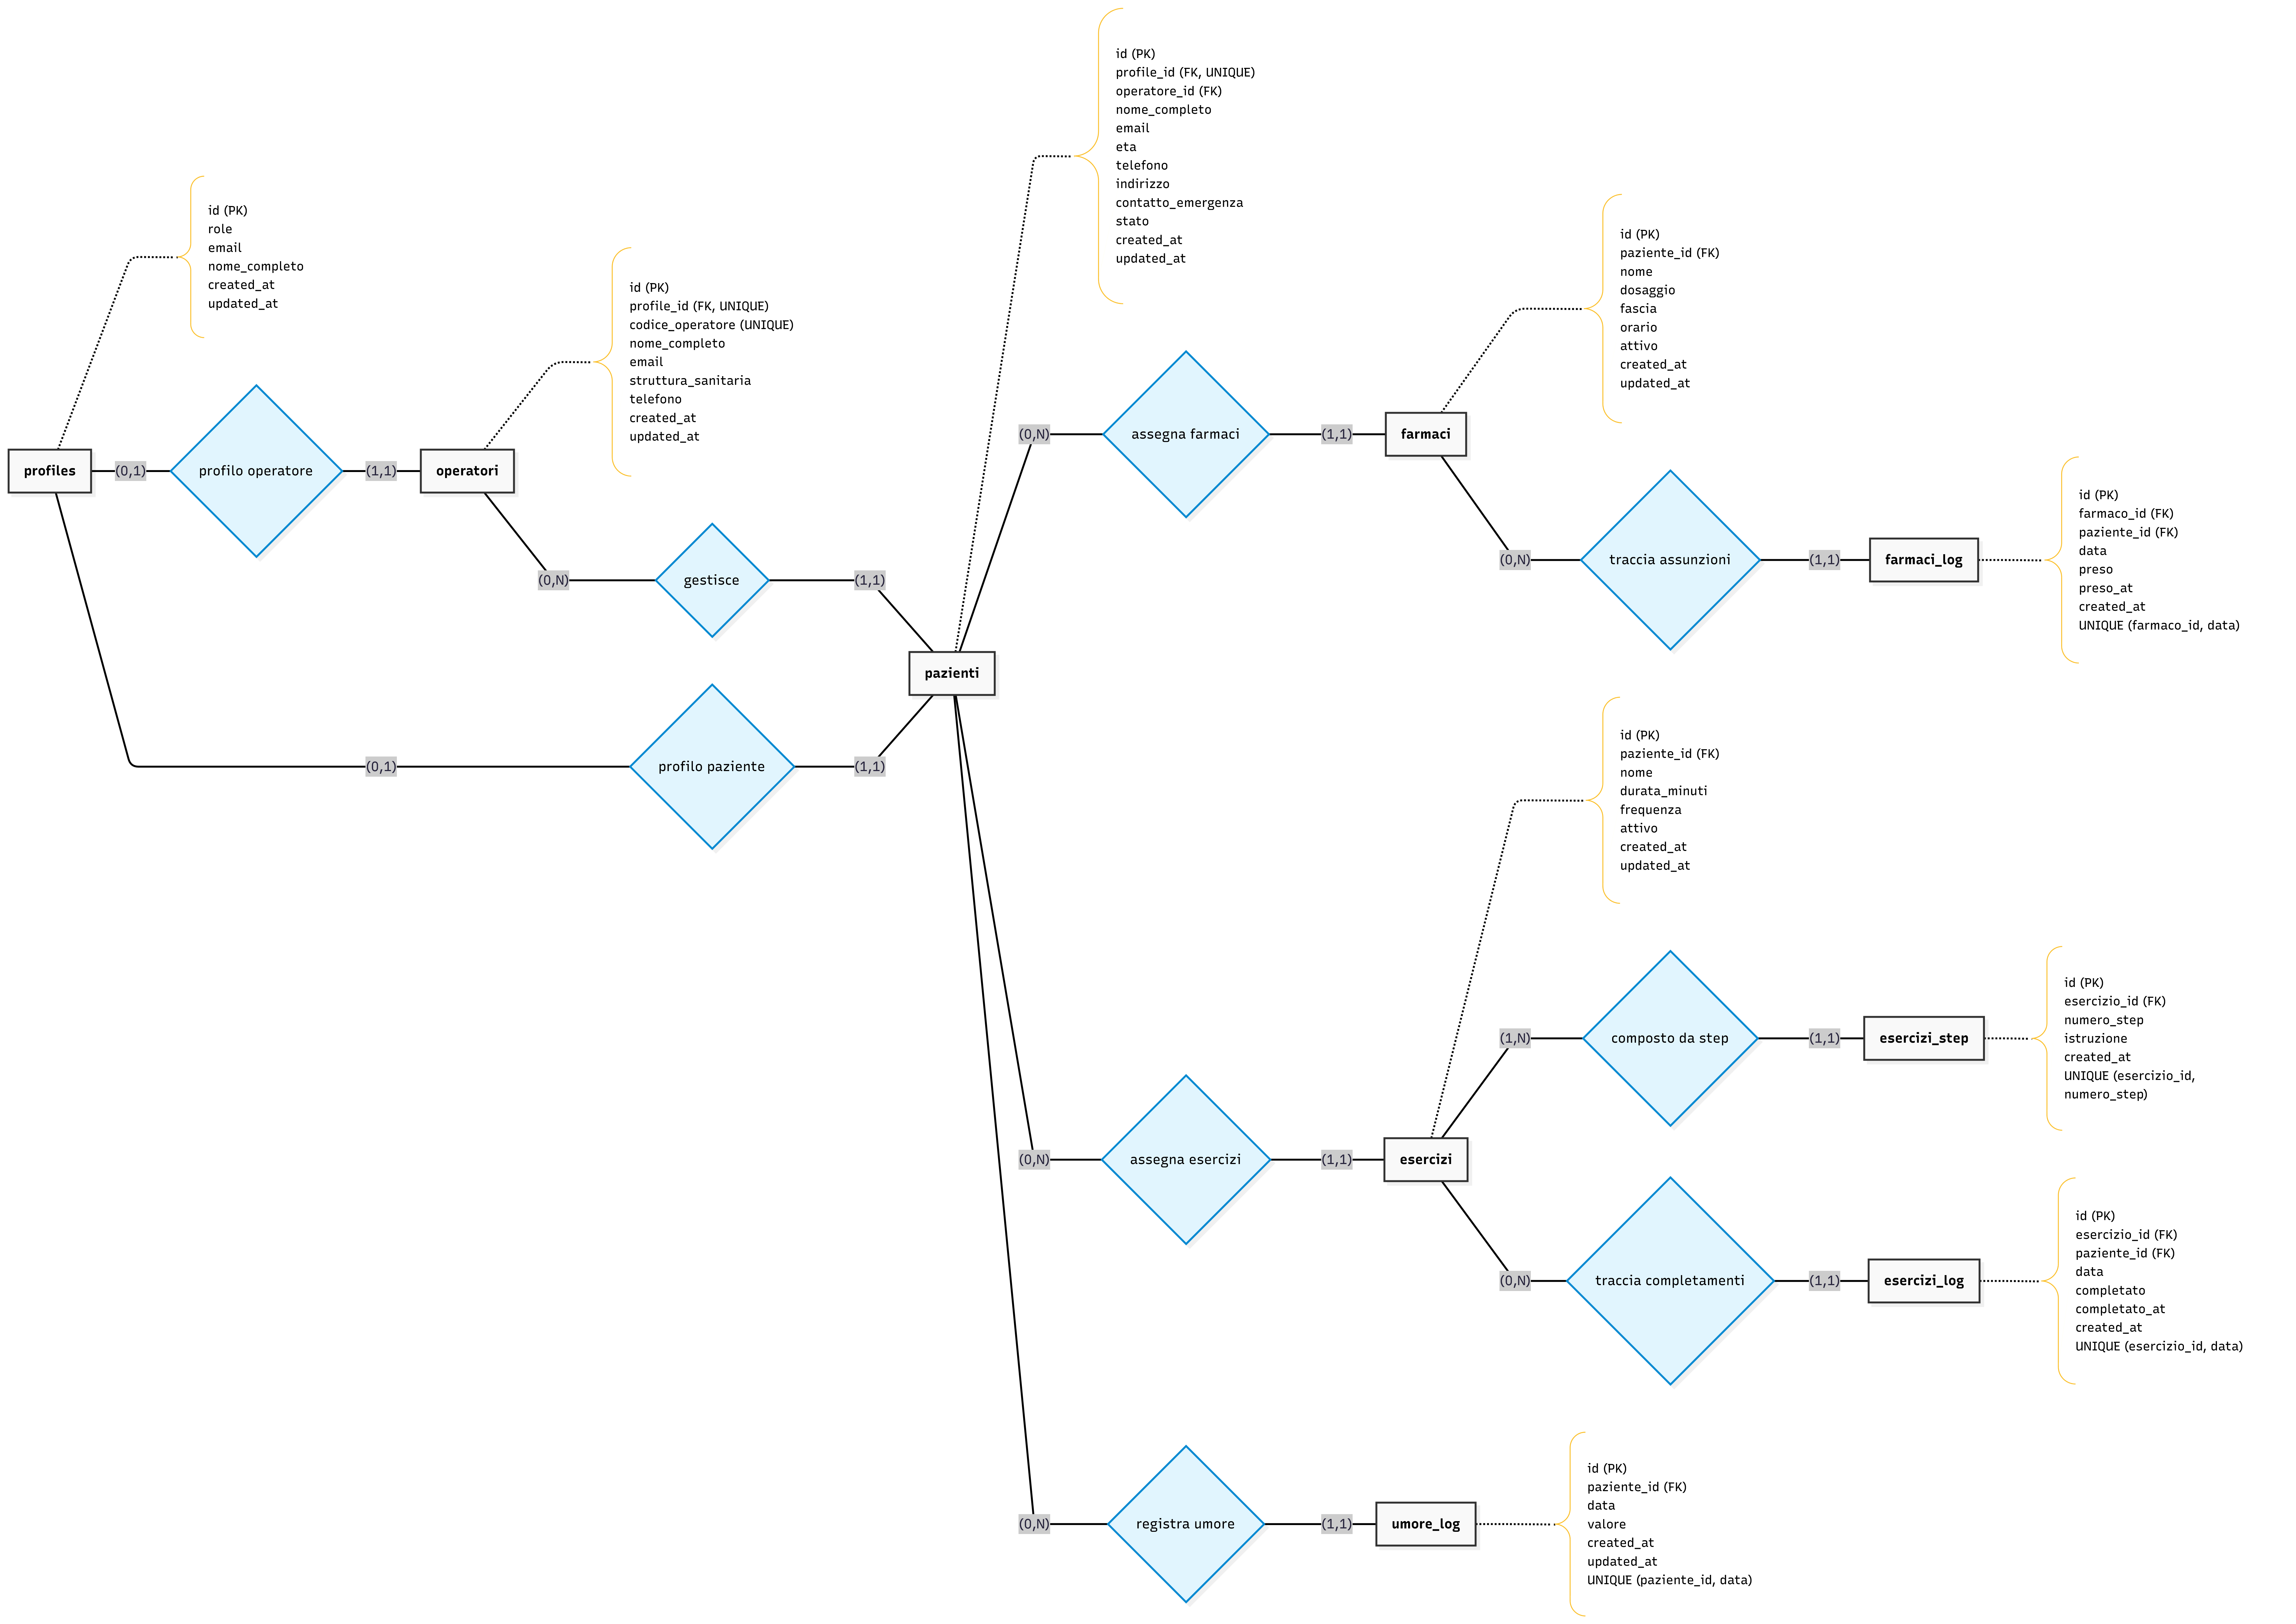
\includegraphics[width=\textwidth,height=0.72\textheight,keepaspectratio]{diagrams/01_eer.png}
\caption{Diagramma EER}
\label{fig:eer}
\end{figure}

\paragraph{Entita' principali}
\begin{itemize}
    \item \textbf{\texttt{profiles}:} profilo applicativo collegato a \texttt{auth.users}. Contiene ruolo, email e nome completo.
    \item \textbf{\texttt{operatori}:} dati dell'operatore sanitario, incluso codice operatore e struttura sanitaria.
    \item \textbf{\texttt{pazienti}:} dati del paziente, operatore assegnato, contatti e stato clinico.
    \item \textbf{\texttt{farmaci}:} farmaci assegnati al paziente, con dosaggio, orario, fascia e stato attivo.
    \item \textbf{\texttt{farmaci\_log}:} registro giornaliero dell'assunzione dei farmaci.
    \item \textbf{\texttt{esercizi}:} esercizi fisici assegnati al paziente.
    \item \textbf{\texttt{esercizi\_step}:} passaggi guidati che compongono un esercizio.
    \item \textbf{\texttt{esercizi\_log}:} registro giornaliero degli esercizi completati.
    \item \textbf{\texttt{umore\_log}:} registrazione giornaliera dell'umore del paziente.
\end{itemize}

\newpage
\subsection{Modello Relazionale}

Il modello relazionale descrive la struttura logica della base di dati, derivato dal diagramma EER. Le tabelle, le chiavi primarie (PK), le chiavi esterne (FK) e i vincoli di integrità referenziale sono rappresentati nel seguente schema:

\begin{figure}[H]
\centering
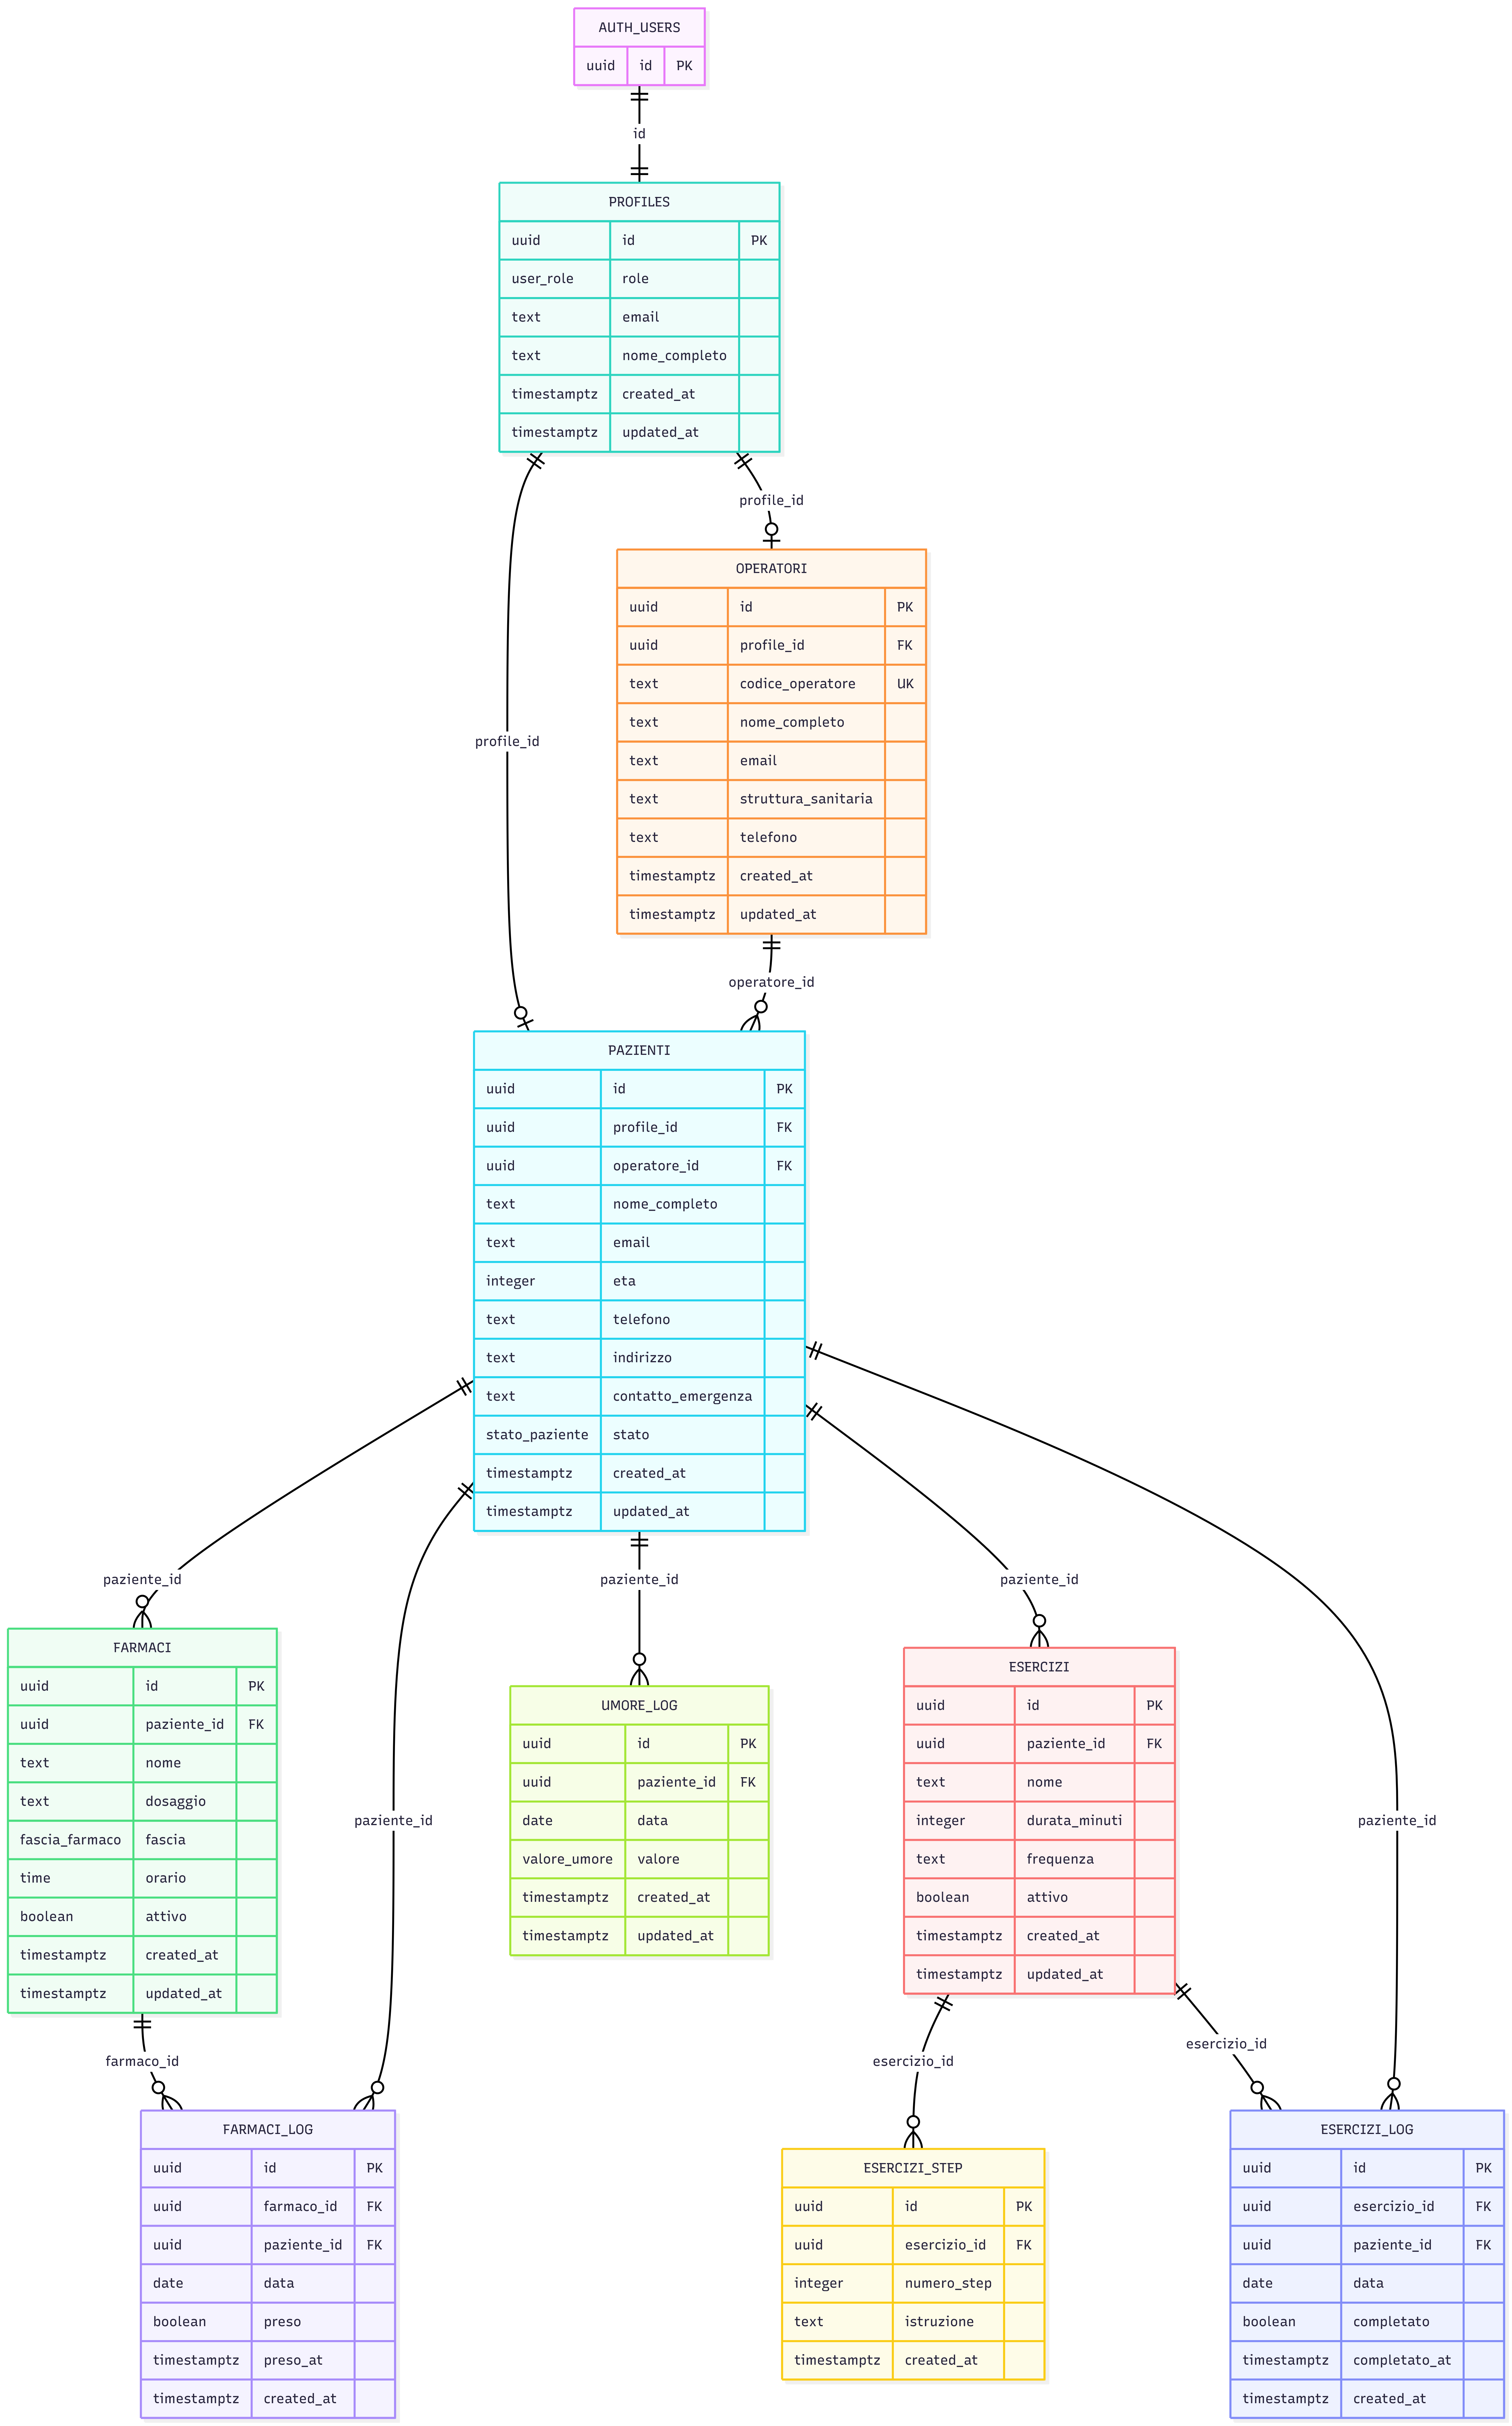
\includegraphics[width=\textwidth,height=0.72\textheight,keepaspectratio]{diagrams/02_modello_relazionale.png}
\caption{Diagramma del modello relazionale con tabelle, PK e FK}
\label{fig:relazionale}
\end{figure}

\subsection{Stima Dimensionale del Database}

\subsubsection{Stima per entita'}
\begin{table}[H]
\centering
\footnotesize
\renewcommand{\arraystretch}{1.25}
\begin{tabular}{|l|r|p{8cm}|}
\hline
\textbf{Tabella} & \textbf{Byte/riga stimati} & \textbf{Note} \\
\hline
profiles & 128 & UUID, ruolo, email, nome e timestamp \\
\hline
operatori & 384 & Dati professionali, codice operatore e contatti \\
\hline
pazienti & 512 & Dati anagrafici, stato e contatto emergenza \\
\hline
farmaci & 208 & Nome, dosaggio, fascia, orario e FK \\
\hline
farmaci\_log & 96 & FK, data, booleano e timestamp \\
\hline
esercizi & 192 & Nome, durata, frequenza e FK \\
\hline
esercizi\_step & 320 & Numero step e istruzione testuale \\
\hline
esercizi\_log & 96 & FK, data, booleano e timestamp \\
\hline
umore\_log & 80 & Data e valore enum testuale \\
\hline
\end{tabular}
\caption{Stima della dimensione media per riga}
\label{tab:stima-byte}
\end{table}

\subsubsection{Tabella di popolamento e crescita}
\begin{table}[H]
\centering
\footnotesize
\renewcommand{\arraystretch}{1.25}
\begin{tabular}{|l|r|r|r|r|}
\hline
\textbf{Tabella} & \textbf{Righe iniziali} & \textbf{Crescita annua} & \textbf{Byte/riga} & \textbf{Dimensione annua stimata} \\
\hline
profiles & 105 & 20 & 128 & $\sim$ 16 KB \\
\hline
operatori & 5 & 1 & 384 & $\sim$ 2 KB \\
\hline
pazienti & 100 & 20 & 512 & $\sim$ 60 KB \\
\hline
farmaci & 500 & 100 & 208 & $\sim$ 122 KB \\
\hline
farmaci\_log & 4.500 & 182.500 & 96 & $\sim$ 17,9 MB \\
\hline
esercizi & 300 & 60 & 192 & $\sim$ 67 KB \\
\hline
esercizi\_step & 900 & 180 & 320 & $\sim$ 337 KB \\
\hline
esercizi\_log & 3.000 & 109.500 & 96 & $\sim$ 10,8 MB \\
\hline
umore\_log & 3.000 & 36.500 & 80 & $\sim$ 3,0 MB \\
\hline
\multicolumn{4}{|r|}{\textbf{Totale dopo un anno}} & $\sim$ \textbf{32,3 MB} \\
\hline
\end{tabular}
\caption{Stima del popolamento e della crescita annua del database}
\label{tab:popolamento}
\end{table}

\subsection{Modello di Visibilita'}

Il modello di visibilità definisce le policy di accesso ai dati in base al ruolo dell'utente autenticato. Il sistema implementa un modello RBAC (Role-Based Access Control) a due livelli: ruolo (operatore vs paziente) e ownership (ogni utente accede solo ai dati di propria competenza).

\begin{figure}[H]
\centering
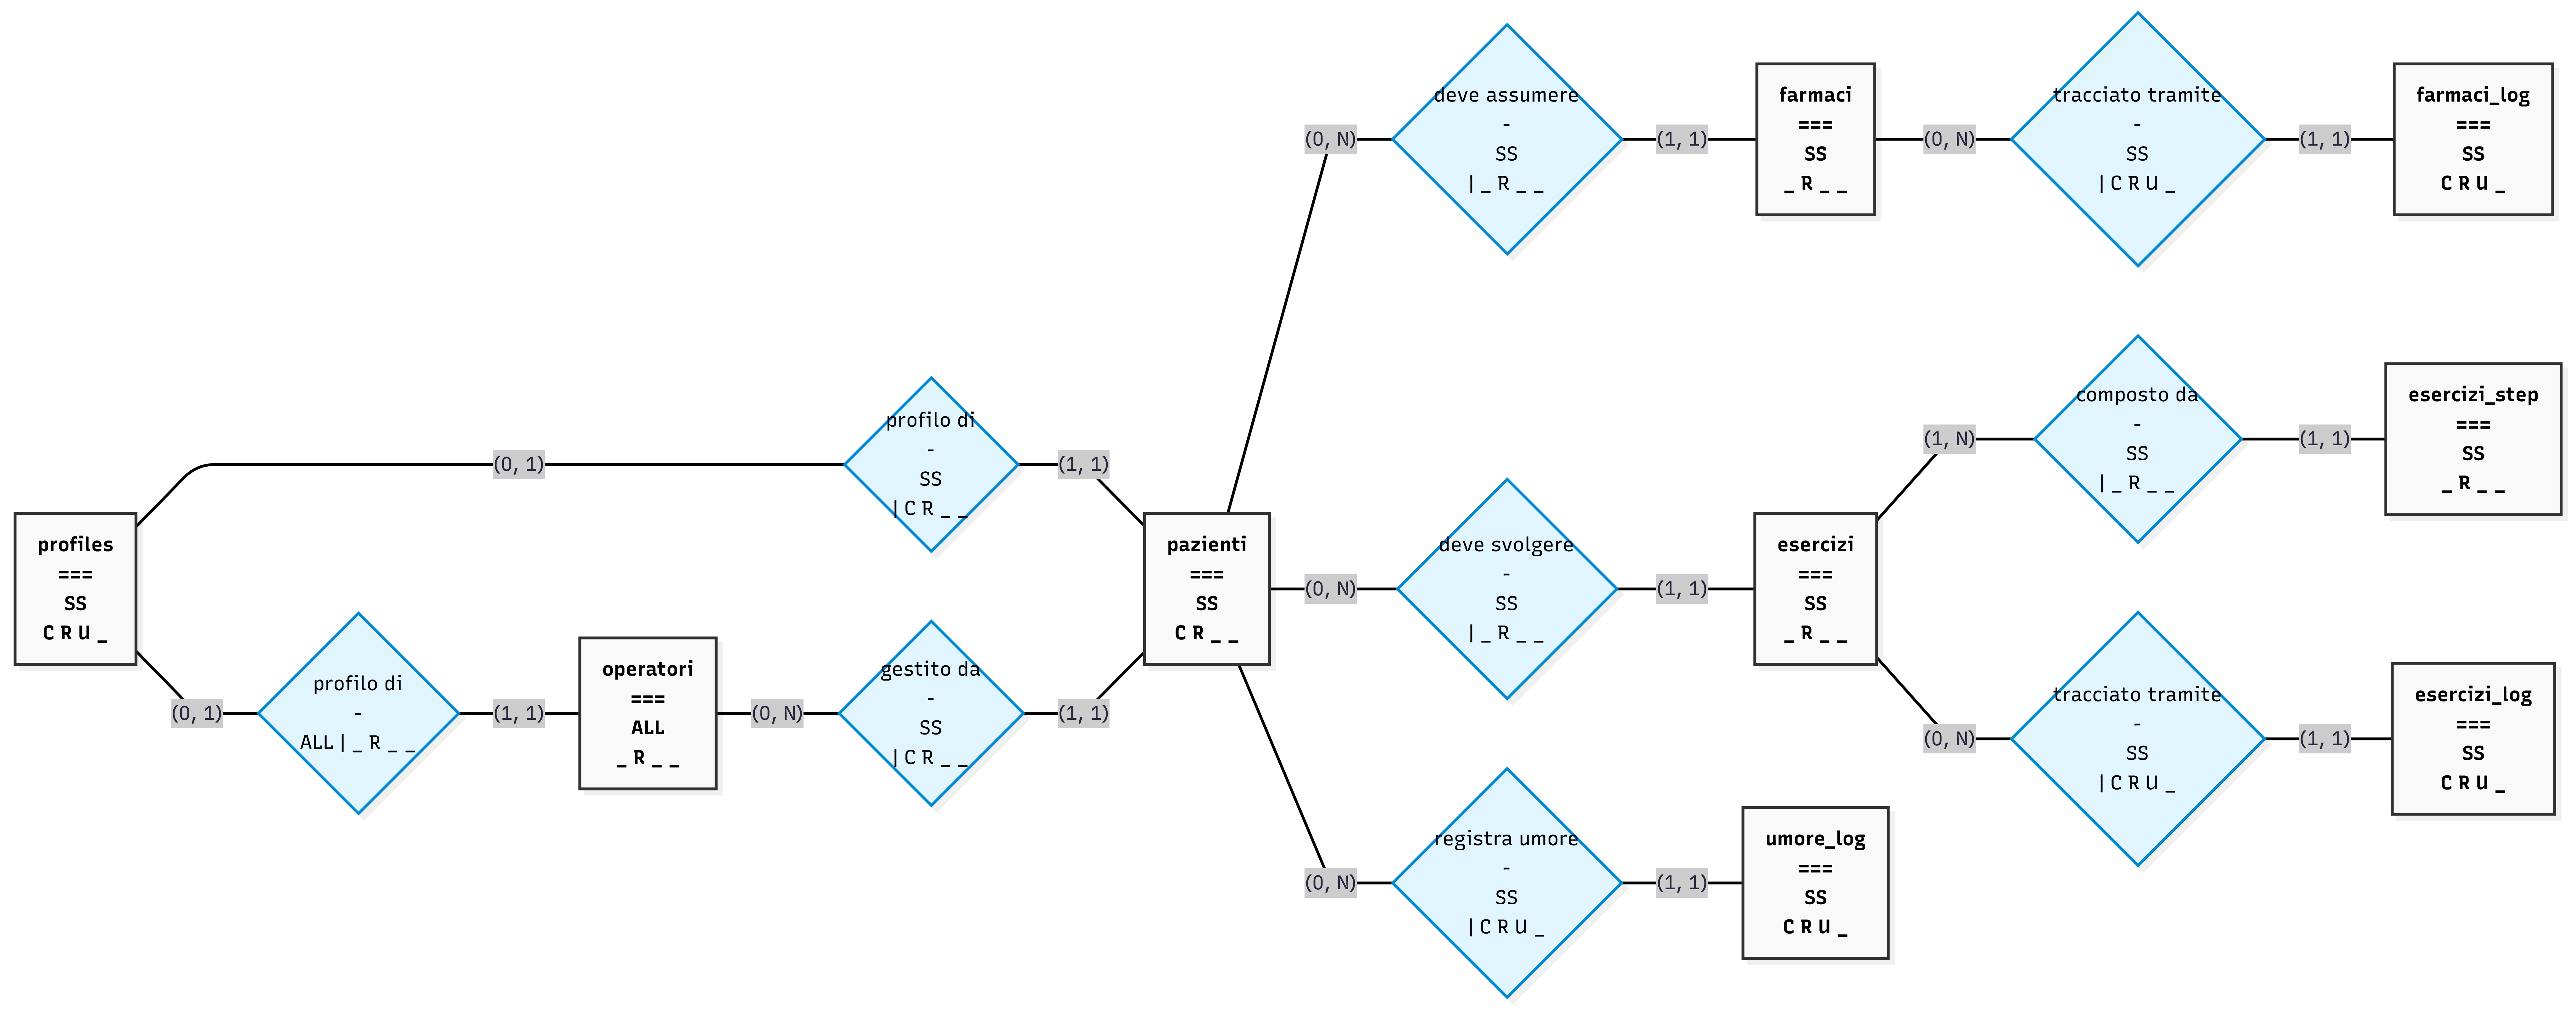
\includegraphics[width=\textwidth,height=0.72\textheight,keepaspectratio]{diagrams/03a_modello_visibilita_paziente.png}
\caption{Modello di visibilita' RLS per il paziente}
\label{fig:visibilita-paziente}
\end{figure}

\begin{figure}[H]
\centering
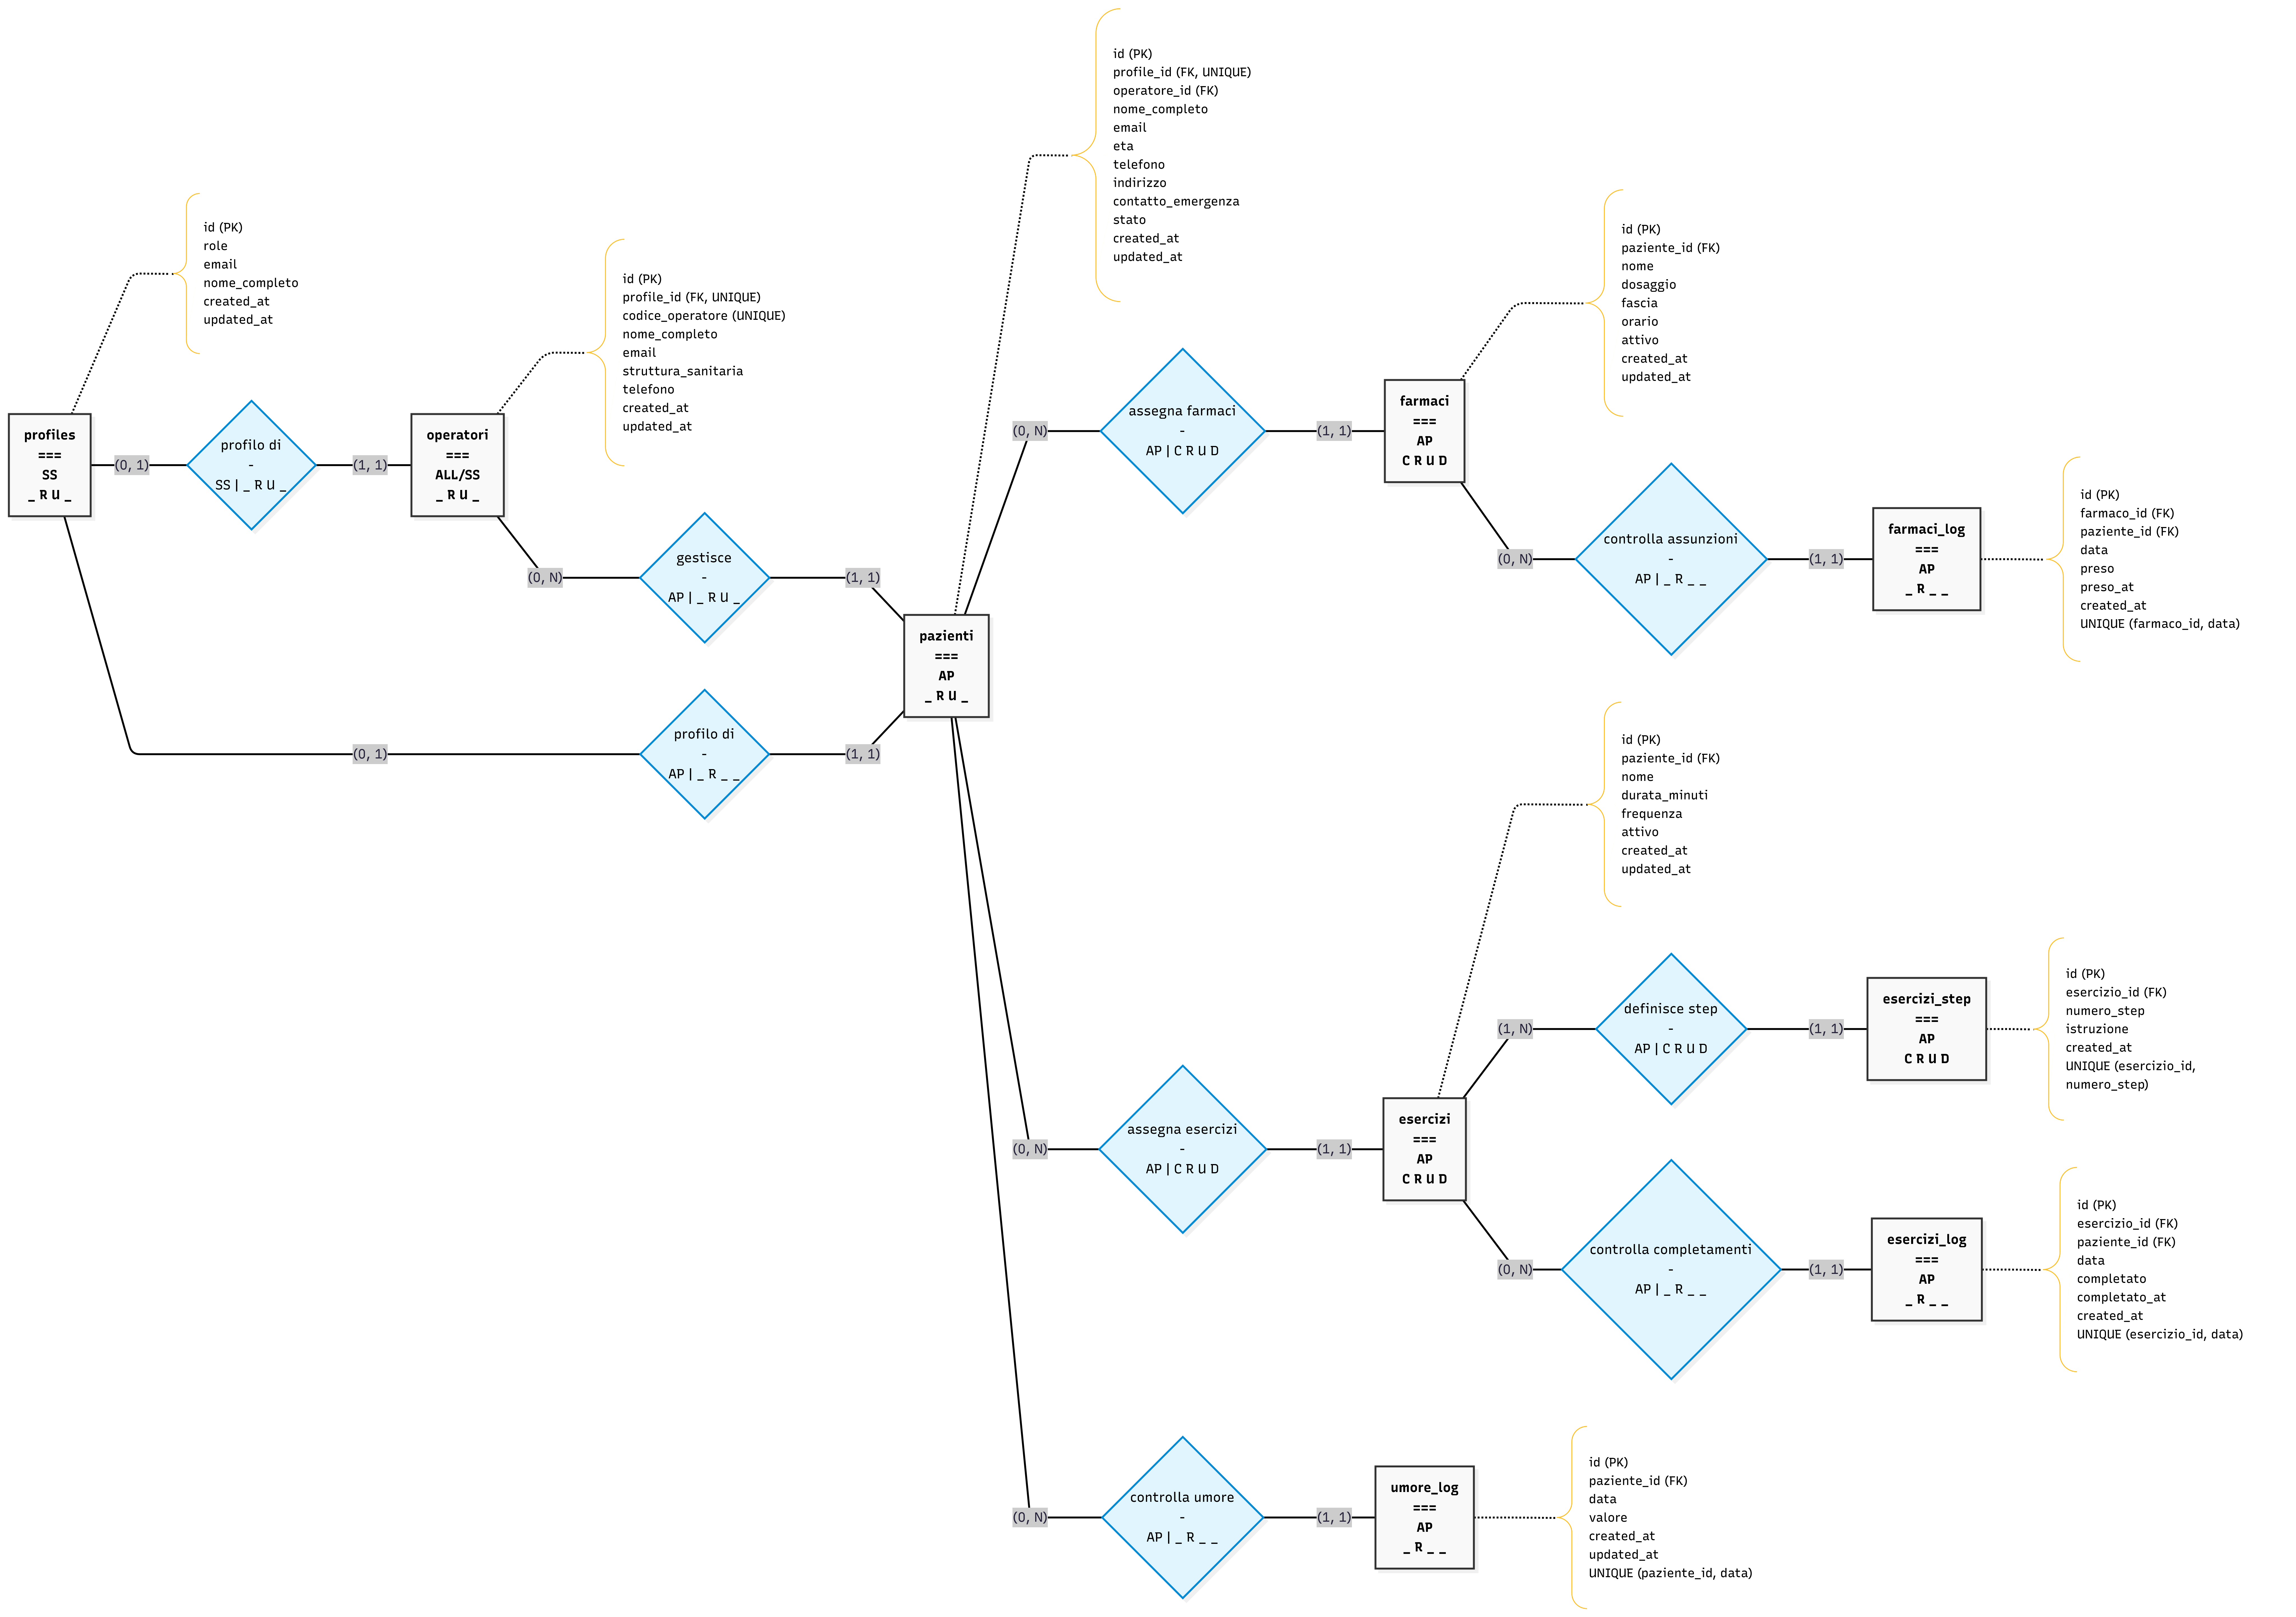
\includegraphics[width=\textwidth,height=0.72\textheight,keepaspectratio]{diagrams/03b_modello_visibilita_operatore.png}
\caption{Modello di visibilita' RLS per l'operatore}
\label{fig:visibilita-operatore}
\end{figure}

\begin{table}[H]
\centering
\footnotesize
\renewcommand{\arraystretch}{1.25}
\begin{tabular}{|p{3.2cm}|c|c|c|c|c|c|c|c|}
\hline
\multirow{2}{*}{\textbf{Risorsa}} & \multicolumn{4}{c|}{\textbf{Operatore}} & \multicolumn{4}{c|}{\textbf{Paziente}} \\
\cline{2-9}
 & C & R & U & D & C & R & U & D \\
\hline
profiles &  & X & X &  &  & X & X &  \\
\hline
operatori &  & X & X &  &  & X &  &  \\
\hline
pazienti &  & X & X &  & X & X &  &  \\
\hline
farmaci & X & X & X & X &  & X &  &  \\
\hline
farmaci\_log &  & X &  &  & X & X & X &  \\
\hline
esercizi & X & X & X & X &  & X &  &  \\
\hline
esercizi\_step & X & X & X & X &  & X &  &  \\
\hline
esercizi\_log &  & X &  &  & X & X & X &  \\
\hline
umore\_log &  & X &  &  & X & X & X &  \\
\hline
\end{tabular}
\caption{Matrice CRUD di visibilita' per ruolo}
\label{tab:visibilita}
\end{table}

\newpage

\section{Modello di Navigazione}

Il modello di navigazione e' stato ricavato dalla struttura reale di \texttt{src/app}. In Next.js App Router ogni cartella che contiene \texttt{page.tsx} diventa una pagina visitabile; per questo motivo il diagramma seguente non descrive funzionalita' ipotetiche, ma solo route presenti nel codice.

\subsection{Legenda}

\begin{table}[H]
\centering
\renewcommand{\arraystretch}{1.25}
\begin{tabular}{|c|p{10cm}|}
\hline
\textbf{Sigla} & \textbf{Significato} \\
\hline
VP & Vista pubblica, accessibile senza autenticazione. \\
\hline
VF & Vista di form, usata per login o registrazione. \\
\hline
VD & Vista dashboard o vista di riepilogo. \\
\hline
VG & Vista gestionale, usata per modificare dati o configurazioni. \\
\hline
VA & Vista assistita per il paziente, con percorso semplice e pochi pulsanti. \\
\hline
API & Route non navigabile come pagina, usata dal codice applicativo. \\
\hline
\end{tabular}
\caption{Legenda del modello di navigazione}
\label{tab:legenda-navigazione}
\end{table}

\subsection{Albero di navigazione reale}

\begin{figure}[H]
\centering
\resizebox{0.98\textwidth}{!}{
\begin{tikzpicture}[
    route/.style={rectangle, draw=aliceblue, fill=alicelight, thick, rounded corners=3pt, text width=3.7cm, minimum height=0.85cm, align=center, font=\scriptsize},
    role/.style={rectangle, draw=alicegreen, fill=alicegreen!10, thick, rounded corners=3pt, text width=3.4cm, minimum height=0.85cm, align=center, font=\scriptsize\bfseries},
    api/.style={rectangle, draw=aliceorange, fill=aliceorange!10, thick, rounded corners=3pt, text width=4cm, minimum height=0.85cm, align=center, font=\scriptsize},
    line/.style={thick, color=aliceblue, -{Stealth[length=2.3mm]}},
    apiLine/.style={thick, dashed, color=aliceorange, -{Stealth[length=2.3mm]}},
]

\node[route] (home) at (0, 0) {\texttt{/}\\Landing\\VP};

\node[role] (opArea) at (-5.2, -1.55) {Area Operatore};
\node[role] (pzArea) at (5.2, -1.55) {Area Paziente};
\draw[line] (home) -- (opArea);
\draw[line] (home) -- (pzArea);

\node[route] (opLogin) at (-8.3, -3.2) {\texttt{/operatore/login}\\Login\\VF};
\node[route] (opReg) at (-5.2, -3.2) {\texttt{/operatore/registrati}\\Registrazione\\VF};
\node[route] (opDash) at (-2.1, -3.2) {\texttt{/operatore/dashboard}\\Dashboard\\VD};
\draw[line] (opArea) -- (opLogin);
\draw[line] (opArea) -- (opReg);
\draw[line] (opArea) -- (opDash);

\node[route] (opDetail) at (-2.1, -4.9) {\texttt{/operatore/dashboard/pazienti/[id]}\\Dettaglio paziente\\VD};
\node[route] (opManage) at (-2.1, -6.6) {\texttt{?tab=gestisci}\\Gestione dati, farmaci, esercizi\\VG};
\node[api] (aiApi) at (-6.7, -5.75) {\texttt{/api/ai/suggerimento-operatore}\\Suggerimento AI\\API};
\draw[line] (opDash) -- (opDetail);
\draw[line] (opDetail) -- (opManage);
\draw[apiLine] (opDetail) -- (aiApi);

\node[route] (pzLogin) at (2.1, -3.2) {\texttt{/paziente/login}\\Login\\VF};
\node[route] (pzReg) at (5.2, -3.2) {\texttt{/paziente/registrati}\\Registrazione\\VF};
\node[route] (pzHome) at (8.3, -3.2) {\texttt{/paziente/home}\\Home\\VA};
\draw[line] (pzArea) -- (pzLogin);
\draw[line] (pzArea) -- (pzReg);
\draw[line] (pzArea) -- (pzHome);

\node[route] (pzMood) at (4.3, -4.9) {\texttt{/paziente/umore}\\Umore\\VA};
\node[route] (pzEx) at (7.4, -4.9) {\texttt{/paziente/esercizi}\\Esercizi\\VA};
\node[route] (pzMed) at (10.5, -4.9) {\texttt{/paziente/farmaci}\\Farmaci\\VA};
\draw[line] (pzHome) -- (pzMood);
\draw[line] (pzHome) -- (pzEx);
\draw[line] (pzHome) -- (pzMed);

\end{tikzpicture}
}
\caption{Albero di navigazione aggiornato alla struttura reale delle pagine}
\label{fig:navigazione-reale}
\end{figure}

\subsection{Descrizione delle viste}

\subsubsection{Area comune}
\begin{itemize}
    \item \textbf{\texttt{/}:} pagina iniziale. Presenta l'accesso alle due aree del sistema. Se l'utente e' gia' autenticato, il file \texttt{proxy.ts} lo reindirizza alla home corretta in base al ruolo.
\end{itemize}

\subsubsection{Area operatore}
\begin{itemize}
    \item \textbf{\texttt{/operatore/login}:} form di accesso per l'operatore sanitario.
    \item \textbf{\texttt{/operatore/registrati}:} form di registrazione dell'operatore.
    \item \textbf{\texttt{/operatore/dashboard}:} vista principale dell'operatore con elenco pazienti, ricerca, filtri e metriche sintetiche.
    \item \textbf{\texttt{/operatore/dashboard/pazienti/[id]}:} dettaglio del paziente con dati anagrafici, farmaci, esercizi, umore, storico settimanale e suggerimento AI.
    \item \textbf{\texttt{?tab=gestisci}:} stato della pagina di dettaglio, non nuova route. Serve a modificare dati, farmaci ed esercizi.
\end{itemize}

\subsubsection{Area paziente}
\begin{itemize}
    \item \textbf{\texttt{/paziente/login}:} form di accesso del paziente.
    \item \textbf{\texttt{/paziente/registrati}:} form di registrazione del paziente.
    \item \textbf{\texttt{/paziente/home}:} home semplificata con tre scelte principali.
    \item \textbf{\texttt{/paziente/umore}:} registrazione o aggiornamento dell'umore giornaliero.
    \item \textbf{\texttt{/paziente/esercizi}:} elenco degli esercizi assegnati e percorso guidato step-by-step.
    \item \textbf{\texttt{/paziente/farmaci}:} elenco dei farmaci del giorno, divisi per fascia oraria, con conferma di assunzione.
\end{itemize}

\subsection{Regole di protezione e reindirizzamento}

La navigazione privata viene controllata dal file \texttt{src/proxy.ts}. Il proxy legge la sessione Supabase e applica poche regole:

\begin{itemize}
    \item utenti non autenticati verso \texttt{/operatore/dashboard} vengono mandati a \texttt{/operatore/login};
    \item utenti non autenticati verso pagine private \texttt{/paziente/} vengono mandati a \texttt{/paziente/login};
    \item utenti autenticati sulla landing vengono mandati alla home del proprio ruolo;
    \item utenti autenticati sulle pagine pubbliche di login o registrazione vengono reindirizzati alla propria area.
\end{itemize}

\subsection{Principi di navigazione}

\begin{enumerate}
    \item \textbf{Separazione per ruolo:} operatore e paziente hanno percorsi distinti.
    \item \textbf{Percorso breve per il paziente:} dalla home paziente si arriva a umore, esercizi e farmaci con un solo click.
    \item \textbf{Dashboard unica per l'operatore:} l'operatore parte dalla dashboard e poi entra nel dettaglio del paziente.
    \item \textbf{Nessuna pagina non implementata:} il modello contiene solo route realmente presenti nel codice.
\end{enumerate}

\newpage

\section{Modello Architetturale}

A.L.I.C.E. e' una web application full-stack basata su \textbf{Next.js App Router} e \textbf{Supabase}. Il progetto non usa un application server separato: Next.js gestisce pagine, componenti server, componenti client, Server Actions, route API e proxy; Supabase gestisce autenticazione, database PostgreSQL, API PostgREST e Row Level Security.

\subsection{Architettura hardware}

L'architettura hardware e' volutamente leggera. Gli utenti accedono tramite browser, mentre il codice applicativo viene eseguito su un ambiente serverless compatibile con Next.js. I dati persistenti e le sessioni sono gestiti da Supabase; il suggerimento AI viene generato tramite Groq API.

\begin{table}[H]
\centering
\renewcommand{\arraystretch}{1.25}
\begin{tabularx}{\textwidth}{|l|l|X|}
\hline
\textbf{Componente} & \textbf{Servizio} & \textbf{Responsabilita'} \\
\hline
Client & Browser web & Visualizzazione interfaccia e invio azioni utente. \\
\hline
Web app & Next.js serverless & Rendering, routing, Server Actions, proxy e route API. \\
\hline
Backend gestito & Supabase & Auth, PostgreSQL, PostgREST e policy RLS. \\
\hline
Servizio AI & Groq API & Generazione del suggerimento testuale per l'operatore. \\
\hline
\end{tabularx}
\caption{Componenti hardware e servizi esterni}
\label{tab:arch-hw}
\end{table}

\subsection{Modello architetturale}

Il modello architetturale non e' un MVC classico. La separazione delle responsabilita' e' ottenuta tramite il modello di Next.js App Router:

\begin{itemize}
    \item le \textbf{pagine} definiscono le viste raggiungibili dall'utente;
    \item i \textbf{Server Components} caricano dati e preparano la UI lato server;
    \item i \textbf{Client Components} gestiscono interazioni complesse nel browser;
    \item le \textbf{Server Actions} gestiscono mutazioni come login, registrazione, farmaci ed esercizi;
    \item il \textbf{proxy} gestisce sessione e redirect delle aree private;
    \item Supabase rappresenta il livello dati e applica le policy di visibilita'.
\end{itemize}

Questa architettura riduce il numero di file necessari rispetto a un backend separato e mantiene la logica vicino alle pagine che la utilizzano.

\subsection{Architettura software}

\begin{figure}[H]
\centering
\resizebox{0.98\textwidth}{!}{
\begin{tikzpicture}[
    layer/.style={rectangle, draw=aliceblue, fill=alicelight, thick, rounded corners=4pt, minimum width=11cm, minimum height=1.35cm, align=center},
    comp/.style={rectangle, draw=gray, fill=white, thick, rounded corners=3pt, minimum width=2.7cm, minimum height=0.75cm, align=center, font=\scriptsize},
    ext/.style={rectangle, draw=aliceorange, fill=aliceorange!10, thick, rounded corners=3pt, minimum width=4.2cm, minimum height=0.85cm, align=center, font=\scriptsize\bfseries},
    line/.style={thick, color=aliceblue, -{Stealth[length=2.5mm]}},
]

\node[layer] (browser) at (0, 0) {Browser: Operatore e Paziente};

\node[layer] (next) at (0, -2) {};
\node[comp] at (-3.6, -2) {App Router\\pagine e layout};
\node[comp] at (-1.2, -2) {Server\\Components};
\node[comp] at (1.2, -2) {Client\\Components};
\node[comp] at (3.6, -2) {\texttt{proxy.ts}\\redirect};

\node[layer] (server) at (0, -4) {};
\node[comp] at (-2.8, -4) {Server Actions\\CRUD e auth};
\node[comp] at (0, -4) {Route Handler\\AI};
\node[comp] at (2.8, -4) {Helper\\\texttt{src/lib}};

\node[ext] (supabase) at (-3.0, -6) {Supabase\\Auth + PostgreSQL + RLS};
\node[ext] (groq) at (3.0, -6) {Groq API\\Suggerimento operatore};

\draw[line] (browser) -- (next);
\draw[line] (next) -- (server);
\draw[line] (server) -- (supabase);
\draw[line] (server) -- (groq);
\end{tikzpicture}
}
\caption{Architettura software a livelli del sistema A.L.I.C.E.}
\label{fig:architettura-software}
\end{figure}

\subsection{Responsabilita' dei livelli}

\begin{table}[H]
\centering
\renewcommand{\arraystretch}{1.25}
\begin{tabularx}{\textwidth}{|l|X|}
\hline
\textbf{Livello} & \textbf{Responsabilita'} \\
\hline
Presentazione & Componenti React, form, dashboard, card e pagine semplificate del paziente. \\
\hline
Navigazione & App Router per le route e \texttt{proxy.ts} per redirect e sessione. \\
\hline
Logica applicativa & Server Actions, pagine server e helper in \texttt{src/lib}. \\
\hline
Dati & Tabelle Supabase, funzioni SQL, trigger e policy RLS. \\
\hline
Integrazione AI & Route \texttt{/api/ai/suggerimento-operatore}, chiamata server-side a Groq. \\
\hline
\end{tabularx}
\caption{Responsabilita' dei livelli software}
\label{tab:livelli-software}
\end{table}

\subsection{Stack tecnologico}

\begin{table}[H]
\centering
\renewcommand{\arraystretch}{1.25}
\begin{tabularx}{\textwidth}{|l|l|X|}
\hline
\textbf{Tecnologia} & \textbf{Versione} & \textbf{Uso nel progetto} \\
\hline
\texttt{next} & 16.1.6 & Framework full-stack, App Router, build e proxy. \\
\hline
\texttt{react} / \texttt{react-dom} & 19.2.3 & Componenti dell'interfaccia utente. \\
\hline
\texttt{@supabase/ssr} & 0.8.0 & Client Supabase compatibile con server, client e proxy. \\
\hline
\texttt{typescript} & 5.x & Tipizzazione del codice applicativo. \\
\hline
CSS Modules / CSS globale & n.d. & Stile delle pagine senza librerie UI esterne. \\
\hline
Groq API & via \texttt{fetch} & Suggerimento AI lato server. \\
\hline
\end{tabularx}
\caption{Stack tecnologico realmente presente nel progetto}
\label{tab:stack-tecnologico}
\end{table}

\subsection{DBMS, browser e sistemi supportati}

Il DBMS e' PostgreSQL tramite Supabase. Il codice applicativo usa il client Supabase per leggere e scrivere dati, mentre le regole RLS nel database impediscono l'accesso a dati non autorizzati. L'applicazione e' fruibile da browser moderni su Windows, macOS, Linux, Android e iPadOS. Per il paziente e' consigliato un tablet o un PC con schermo ampio; per l'operatore e' sufficiente un PC, laptop o tablet.

\newpage

\section{Aspetti Implementativi}

Gli aspetti implementativi descrivono come l'architettura viene tradotta in file e responsabilita' concrete. Il progetto usa una struttura semplice, coerente con Next.js App Router: le pagine stanno in \texttt{src/app}, i componenti riutilizzabili in \texttt{src/components}, le funzioni di supporto in \texttt{src/lib} e la protezione della navigazione in \texttt{src/proxy.ts}.

\subsection{Struttura del progetto}

\begin{figure}[H]
\centering
\resizebox{0.98\textwidth}{!}{
\begin{tikzpicture}[
    root/.style={rectangle, draw=aliceblue, fill=aliceblue!12, thick, rounded corners=4pt, minimum width=3.4cm, minimum height=0.9cm, align=center, font=\small\bfseries},
    folder/.style={rectangle, draw=alicegreen, fill=alicegreen!10, thick, rounded corners=3pt, minimum width=3.5cm, minimum height=0.85cm, align=center, font=\scriptsize\bfseries},
    file/.style={rectangle, draw=gray, fill=gray!8, rounded corners=3pt, minimum width=3.5cm, minimum height=0.75cm, align=center, font=\scriptsize},
    line/.style={thick, color=aliceblue},
]
\node[root] (src) at (0, 0) {\texttt{src}};

\node[folder] (app) at (-5, -1.6) {\texttt{app}\\route e pagine};
\node[folder] (components) at (0, -1.6) {\texttt{components}\\UI riusabile};
\node[folder] (lib) at (5, -1.6) {\texttt{lib}\\helper};
\draw[line] (src) -- (app);
\draw[line] (src) -- (components);
\draw[line] (src) -- (lib);

\node[file] (op) at (-7.2, -3.2) {\texttt{operatore}\\dashboard e actions};
\node[file] (pz) at (-5, -3.2) {\texttt{paziente}\\home, umore, esercizi, farmaci};
\node[file] (api) at (-2.8, -3.2) {\texttt{api/ai}\\route Groq};
\draw[line] (app) -- (op);
\draw[line] (app) -- (pz);
\draw[line] (app) -- (api);

\node[file] (dash) at (-1.2, -3.2) {\texttt{DashboardContent}\\filtri e lista};
\node[file] (card) at (0.9, -3.2) {\texttt{PatientCard}\\riepilogo};
\node[file] (detail) at (3.0, -3.2) {\texttt{PazienteDettaglio}\\tab e gestione};
\draw[line] (components) -- (dash);
\draw[line] (components) -- (card);
\draw[line] (components) -- (detail);

\node[file] (date) at (4.0, -3.2) {\texttt{date.ts}};
\node[file] (form) at (5.3, -3.2) {\texttt{form.ts}};
\node[file] (metrics) at (6.6, -3.2) {\texttt{metriche.ts}};
\draw[line] (lib) -- (date);
\draw[line] (lib) -- (form);
\draw[line] (lib) -- (metrics);

\node[file] (proxy) at (0, -4.8) {\texttt{src/proxy.ts}\\sessione e redirect};
\draw[line] (src) -- (proxy);
\end{tikzpicture}
}
\caption{Struttura implementativa principale del progetto}
\label{fig:struttura-progetto}
\end{figure}

\subsection{Pagine e route}

Le route principali sono separate per ruolo. L'area operatore contiene login, registrazione, dashboard e dettaglio paziente. L'area paziente contiene login, registrazione, home e le tre funzioni giornaliere: umore, esercizi e farmaci. La route \texttt{/api/ai/suggerimento-operatore} non e' una pagina, ma un endpoint server-side richiamato dal dettaglio paziente.

\begin{table}[H]
\centering
\renewcommand{\arraystretch}{1.25}
\footnotesize
\begin{tabularx}{\textwidth}{|p{5.6cm}|X|}
\hline
\textbf{File} & \textbf{Responsabilita'} \\
\hline
\texttt{src/app/operatore/dashboard/page.tsx} & Carica l'operatore, i pazienti assegnati e le metriche di riepilogo. \\
\hline
\texttt{src/app/operatore/dashboard/pazienti/[id]/page.tsx} & Verifica che il paziente appartenga all'operatore e prepara dati di dettaglio. \\
\hline
\texttt{src/app/paziente/home/page.tsx} & Mostra la home semplificata del paziente. \\
\hline
\texttt{src/app/paziente/umore/page.tsx} & Salva o aggiorna l'umore giornaliero. \\
\hline
\texttt{src/app/paziente/esercizi/page.tsx} & Gestisce l'esecuzione guidata e il log degli esercizi. \\
\hline
\texttt{src/app/paziente/farmaci/page.tsx} & Mostra farmaci per fascia e registra l'assunzione. \\
\hline
\end{tabularx}
\caption{Pagine principali}
\label{tab:pagine-implementate}
\end{table}

\subsection{Server Actions e accesso ai dati}

Le Server Actions gestiscono le operazioni che modificano dati: registrazione, login, logout, aggiornamento del paziente, aggiunta o rimozione di farmaci ed esercizi. La scelta delle Server Actions evita controller REST manuali per ogni form e mantiene la logica lato server.

\begin{table}[H]
\centering
\renewcommand{\arraystretch}{1.25}
\begin{tabularx}{\textwidth}{|p{5.8cm}|X|}
\hline
\textbf{File} & \textbf{Operazioni principali} \\
\hline
\texttt{src/app/operatore/actions.ts} & Login, registrazione e logout operatore. \\
\hline
\texttt{src/app/paziente/actions.ts} & Login, registrazione e logout paziente. \\
\hline
\texttt{src/app/operatore/dashboard/pazienti/actions.ts} & Update paziente, create/delete farmaco, create/delete esercizio. \\
\hline
\end{tabularx}
\caption{Server Actions del progetto}
\label{tab:server-actions}
\end{table}

\subsection{Componenti client}

I componenti client sono usati dove serve interazione nel browser. \texttt{DashboardContent.tsx} gestisce ricerca e filtri nella dashboard; \texttt{PatientCard.tsx} visualizza un paziente in forma sintetica; \texttt{PazienteDettaglio.tsx} gestisce tab, modali, form, storico e richiesta del suggerimento AI.

\subsection{Helper di supporto}

Durante il refactoring alcune funzioni ripetute sono state spostate in \texttt{src/lib}. \texttt{date.ts} gestisce la data corrente, \texttt{form.ts} centralizza la lettura dei valori da \texttt{FormData}, \texttt{metriche.ts} calcola percentuali e \texttt{paziente-client.ts} recupera l'id del paziente associato all'utente autenticato.

\subsection{Suggerimento AI}

Il suggerimento AI e' isolato nella route \texttt{src/app/api/ai/suggerimento-operatore/route.ts}. Il client invia dati sintetici e non identificativi; la route usa la chiave \texttt{GROQ\_API\_KEY} lato server, chiama Groq tramite \texttt{fetch} e restituisce una sola frase per l'operatore. Questa separazione evita di inserire la chiave nel browser e mantiene la logica AI fuori dal componente React.

\subsection{Sicurezza}

La sicurezza si basa su Supabase Auth, proxy Next.js e Row Level Security. Il proxy protegge le pagine private e gestisce i redirect; le pagine server controllano che l'operatore acceda solo ai propri pazienti; le policy RLS nel database impediscono letture o modifiche non coerenti con il ruolo.

\newpage

\section{Test}

Per il test del sistema A.L.I.C.E. sono stati utilizzati i seguenti strumenti:

\begin{itemize}
    \item \textbf{Postman} -- Applicazione utilizzata per effettuare test funzionali sulle API di Supabase, verificandone il corretto funzionamento simulando richieste HTTP (GET, POST, PATCH, DELETE) verso gli endpoint REST auto-generati da PostgREST.

    \item \textbf{ESLint} -- Strumento di analisi statica del codice JavaScript/TypeScript, utilizzato per individuare e correggere bug, errori di sintassi e problemi di stile, migliorando la qualità e la coerenza del codice sorgente.

    \item \textbf{Supabase Dashboard (SQL Editor)} -- Interfaccia web fornita da Supabase per eseguire query SQL dirette sul database PostgreSQL, utilizzata per verificare la corretta persistenza dei dati e il funzionamento delle policy Row Level Security.

    \item \textbf{Chrome DevTools} -- Strumenti di sviluppo integrati nel browser Google Chrome, utilizzati per il debug del frontend React, l'analisi delle richieste di rete, il controllo del rendering dei componenti e la verifica della responsività dell'interfaccia.
\end{itemize}

\newpage

\section{Conclusioni}

Il progetto A.L.I.C.E. realizza una piattaforma web semplice per il monitoraggio remoto di pazienti
anziani. La soluzione mette insieme tre aree concrete: farmaci, esercizi fisici e umore quotidiano.
L'operatore usa una dashboard per controllare i pazienti, mentre il paziente usa pagine lineari con
azioni brevi e leggibili.

\subsection{Risultati raggiunti}

\begin{itemize}
    \item \textbf{Separazione dei ruoli:} operatore e paziente hanno pagine, login e percorsi distinti.
    \item \textbf{Dashboard operatore:} l'operatore visualizza pazienti, stato, metriche e dettaglio individuale.
    \item \textbf{Area paziente semplificata:} il paziente accede a umore, esercizi e farmaci partendo da una home con tre scelte principali.
    \item \textbf{Database coerente:} lo schema contiene tabelle dedicate a profili, operatori, pazienti, farmaci, esercizi e log.
    \item \textbf{Navigazione protetta:} il proxy Next.js gestisce i redirect principali in base alla sessione Supabase.
    \item \textbf{Suggerimento AI:} l'operatore puo' ricevere una frase sintetica di supporto basata sui dati del paziente.
\end{itemize}

\subsection{Benefici attesi}

\paragraph{Per il paziente}
\begin{itemize}
    \item interfaccia piu' semplice rispetto a un gestionale sanitario tradizionale;
    \item meno passaggi per registrare umore, farmaci ed esercizi;
    \item conferma immediata delle azioni completate.
\end{itemize}

\paragraph{Per l'operatore}
\begin{itemize}
    \item visione centralizzata dei pazienti seguiti;
    \item controllo piu' rapido di aderenza farmacologica, esercizi e umore;
    \item possibilita' di modificare piano e dati del paziente da una sola pagina.
\end{itemize}

\subsection{Limiti attuali}

Il progetto copre il flusso principale, ma resta una piattaforma didattica. Alcune funzioni sono
volutamente semplici: non sono presenti notifiche automatiche, videochiamate, app mobile nativa o
integrazione con dispositivi medici. Questa scelta mantiene il codice piu' leggibile e adatto alla
presentazione universitaria.

\subsection{Sviluppi futuri}

Possibili miglioramenti futuri sono:

\begin{itemize}
    \item notifiche per ricordare al paziente farmaci ed esercizi;
    \item grafici piu' avanzati per lo storico dell'operatore;
    \item esportazione dei report del paziente;
    \item videochiamata semplificata tra operatore e paziente;
    \item app mobile o Progressive Web App installabile.
\end{itemize}

\newpage

\section{Matrice RACI}

La matrice RACI chiarisce la distribuzione delle responsabilita' tra i membri del gruppo. Le sigle utilizzate sono:

\begin{itemize}
    \item \textbf{R} -- Responsible: esegue l'attivita';
    \item \textbf{A} -- Accountable: approva il risultato;
    \item \textbf{C} -- Consulted: fornisce supporto o revisione;
    \item \textbf{I} -- Informed: viene informato sull'esito.
\end{itemize}

\subsection{Ruoli del team}

\begin{table}[H]
\centering
\renewcommand{\arraystretch}{1.25}
\begin{tabularx}{\textwidth}{|l|X|}
\hline
\textbf{Studente} & \textbf{Responsabilita' prevalente} \\
\hline
Manuel Manna & Coordinamento della relazione, contesto, stato dell'arte, revisione finale. \\
\hline
Alessio Mininni & Implementazione, refactoring, Supabase, architettura software e allineamento codice-documentazione. \\
\hline
Andrius Tamuliunaite & Analisi dei modelli, verifica funzionale, supporto alla navigazione e revisione dei contenuti. \\
\hline
\end{tabularx}
\caption{Ruoli del team}
\label{tab:team-raci}
\end{table}

\subsection{RACI della documentazione}

\begin{table}[H]
\centering
\renewcommand{\arraystretch}{1.25}
\footnotesize
\begin{tabularx}{\textwidth}{|X|c|c|c|}
\hline
\textbf{Attivita'} & \textbf{Manna} & \textbf{Mininni} & \textbf{Tamuliunaite} \\
\hline
Capitolo 1: contesto e obiettivi & A/R & C & C \\
\hline
Capitolo 2: stakeholder, goal e valore & C & C & A/R \\
\hline
Capitolo 3: stato dell'arte e make or buy & A/R & I & C \\
\hline
Capitolo 4: EER, relazionale e visibilita' & C & A/R & C \\
\hline
Capitolo 5: modello di navigazione & C & A/R & C \\
\hline
Capitolo 6: modello architetturale & C & A/R & I \\
\hline
Capitolo 7: aspetti implementativi & I & A/R & C \\
\hline
Capitoli 8-9: test e conclusioni & A & C & R \\
\hline
Revisione finale della relazione & A/R & C & C \\
\hline
\end{tabularx}
\caption{Matrice RACI della documentazione}
\label{tab:raci-documentazione}
\end{table}

\subsection{RACI dello sviluppo}

\begin{table}[H]
\centering
\renewcommand{\arraystretch}{1.25}
\footnotesize
\begin{tabularx}{\textwidth}{|X|c|c|c|}
\hline
\textbf{Attivita'} & \textbf{Manna} & \textbf{Mininni} & \textbf{Tamuliunaite} \\
\hline
Configurazione progetto Next.js & I & A/R & C \\
\hline
Schema Supabase e policy RLS & C & A/R & C \\
\hline
Autenticazione operatore e paziente & I & A/R & C \\
\hline
Dashboard operatore & C & A/R & C \\
\hline
Dettaglio paziente e gestione farmaci/esercizi & C & A/R & C \\
\hline
Pagine paziente: home, umore, esercizi, farmaci & C & A/R & R \\
\hline
Proxy Next.js e protezione navigazione & I & A/R & C \\
\hline
Route AI con Groq & I & A/R & C \\
\hline
Refactoring helper in \texttt{src/lib} & I & A/R & C \\
\hline
Test manuali dei flussi principali & C & C & A/R \\
\hline
\end{tabularx}
\caption{Matrice RACI dello sviluppo}
\label{tab:raci-sviluppo}
\end{table}

\newpage


\end{document}
